\newpage
\appendix
\section{Appendix}

All tables, figures and results can be reproduced with the code in our \href{https://gitlab.gwdg.de/joel.beck/airbnb-oslo}{GitLab Repository}.

\subsection{Image Processing and Modeling} \label{appendix:images}

\subsubsection{Webscraping}

In the first step, the raw image links provided by the data set had to converted to an image format that the neural network is able to work with.

Therefore we first used the \href{https://docs.python-requests.org/en/latest/}{requests} library to get the HTML Source Code of each listing's website.
Next, the \href{https://beautiful-soup-4.readthedocs.io/en/latest/}{beautifulsoup} library served as a convenient HTML parser to find and extract all embedded weblinks that lead to images located on the front page of the listings website.
With this strategy we could extract the first $5$ images for each apartment (if $5$ or more were available) that could be directly accessed from the front page source code.

Finally, we used the \texttt{requests} module again in combination with the \href{https://pillow.readthedocs.io/en/stable/}{pillow} package to decode the source content of all image adresses into two dimensional images.

\subsubsection{Image Transformations}

Before feeding these two dimensional images into the model, we performed some further preprocessing steps.

One very common technique when dealing with images is \emph{Data Augmentation}.
In contrast to classification tasks however, where Data Augmentation is used to expand the training set and improve simultaneously generalization, this approach is not immediately transferable to a regression context since we have to guarantee that the label (i.e. the price) remains unchanged for each image transformation.
Thus, we decided against standard transformations such as rotating the images or manipulating the color composition.

We did use image \emph{cropping}, however, which, in our opinion, is one of the few applicable augmentations in regression contexts.
After resizing all images to $256 \times 256$ pixels we randomly cropped a square area of $224 \times 224$ out of each image in the training set and cropped an equally sized area out of the image \emph{center} in the validation set to avoid any randomness during inference.

At a final step all images were normalized, separately for each color channel.
In case of the pretrained model \texttt{ResNet} we used the same values for normalization that were used during training on the large \texttt{ImageNet} database \citep{russakovsky2015}.
The mean values and standard deviations for each color channel are provided in the \href{https://pytorch.org/vision/stable/models.html}{PyTorch documentation}.

%%%
\begin{figure}[t]
  \centering
  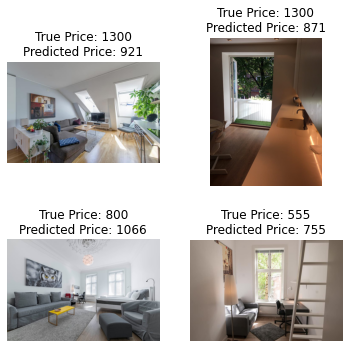
\includegraphics[width=0.5\textwidth]{cnn_examples_small.png}
  \caption{Images from Airbnb Apartments with true and predicted Prices}
  \label{fig:cnn-examples}
\end{figure}
%%%

\subsection{Feature Selection} \label{appendix:feature-selection}

Not all features out of the new combined and extended feature set are equally valuable to the model in terms of predictive power.
In fact, some of the features could not even be transformed to meaningful predictors due to containing e.g. \emph{id} information.
Others were completely redundant in presence of a combination of original and/or manually constructed features and were thus dropped from the feature set.

Before starting the modeling we intended to reduce the feature set even further to avoid strong correlations among the input predictors and possibly improve generalization performance to out-of-sample data.
Thus, we agreed on a two-step strategy.

First, we manually selected features based on three criteria:
%%%
\begin{enumerate}
  \item The variable in consideration and the apartment price must have some connection based on human intuition and background knowledge. For instance, we included variables containing information about the apartment's \emph{size} such as the number of \emph{accomodates}, the number of \emph{bathrooms} and the number of \emph{bedrooms}.
  \item There has to exist some correlation with the price in a bivariate visualization, e.g. a \emph{barplot} in case of categorical predictors or a \emph{scatterplot} in case of numeric features.
  \item Since our dataset was comparably small with roughly $3000$ observations, we had to take care about missing values.
        Therefore, each variable whose missing values could not be imputed in a meaningful and uncontroversial manner was either selected or dropped based on the trade-off of potential data reduction and its additional predictive value.
\end{enumerate}
%%%

Up to this point the feature selection process was solely based on bivariate relationships and self-chosen (arguably arbitrary) selection criteria.
There was a high chance of exluding important predictors that shine in combination with other variables rather than on their own.

Therefore, in a second step, we fitted an auxiliary Linear Regression model with \emph{all} available features (except for the trivial ones such as the \emph{picture url}) and analyzed the absolute magnitude of the coefficients.
Since all variables are standardized, these magnitudes are within the same range and unit-independent, and can thus be compared.

Of course, even this approach is not perfect, as several highly correlated characteristics that have a strong influence on price could lead to rather small estimated individual coefficients due to their joint predictive/explanatory power.
To circumvent this potential issue, we additionally used the \emph{algorithmic} feature selectors provided by the \href{https://scikit-learn.org/stable/index.html}{scikit-learn} library, which (ideally) are able to separate the effects of highly correlated features and select only a small subset of them.

Thereby we focused on two algorithms:
%%%
\begin{itemize}
  \item Principal Component Analysis (\href{https://scikit-learn.org/stable/modules/generated/sklearn.decomposition.PCA.html}{PCA}):
        Reduces dimensionality with the additional benefit of creating \emph{uncorrelated} linear combinations of existing features.
  \item Recursive Feature Selection (\href{https://scikit-learn.org/stable/modules/generated/sklearn.feature_selection.RFE.html}{RFE}):
        Selects subset of original features by leveraging an external estimator (in our case a \emph{Support Vector Regressor}).
        We chose the \texttt{RFE} algorithm for the main analysis since the selected features can be immediately interpreted and the performance on the selected feature set was slightly better compared to \texttt{PCA}.

\end{itemize}
%%%

The influence of the feature selector on the predictive and particularly the generalization performance is discussed in the \emph{Results} section.

\subsection{Price Distribution} \label{appendix:price-distribution}

One key aspect of exploratory data analysis is investigating the \emph{distribution} of the outcome variable.
In our case the price distribution is highly right-skewed with a few very expensive listings pulling the mean and median of the price distribution further away from each other.

Some statistical models such as \emph{Linear Regression} tend to perform better when the outcome distribution is symmetric and approximately normal, whereas some very flexible algorithms like \emph{Neural Networks} do not make any distributional assumptions and are capable of modeling any kind of distribution accurately.
Figure \ref{fig:price-distribution} illustrates an approximate normal distribution can be achieved with a simple logarithmic distribution.

Whereas \emph{all} of the classical models benefitted from the log-transformation resulting in lower error metrics, this was not the case for the Neural Network we used.

In fact, training turned out to be more challenging, since the \emph{magnitude} of the losses by comparing true and predicted price on the logarithmic scale was drastically reduced, leading to smaller gradients and thus smaller weight updates.
This issue could be mitigated to some extent with a larger learning rate.
However, in contrast to the untransformed version, the network still suffered from \emph{vanishing gradients} and \emph{loss plateaus}.

%%%
\begin{figure}[ht]
  \centering
  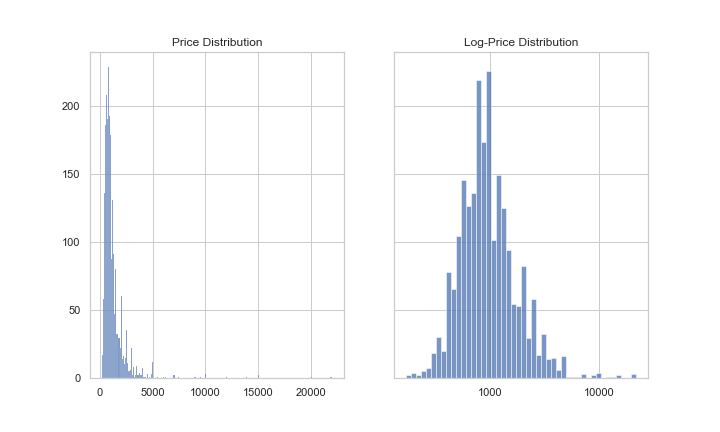
\includegraphics[width=0.8\textwidth]{price_distribution.png}
  \caption{Distribution of Apartment Prices on original and logarithmic Scale}
  \label{fig:price-distribution}
\end{figure}
%%%


\subsection{Neural Network}

\subsubsection{Further (Hyper)-Parameters} \label{appendix:hyperparameters}

\textbf{Optimizer and Weight Decay} \\
We used the popular \texttt{Adam} algorithm \citep{kingma2017} for training the Neural Network.
Compared to vanilla Gradient Descent (with optional momentum) the loss curves during the training process looked much smoother.
Moreover, while pure Gradient Descent slightly benefitted from an additonal weight penalty, neither the classical $L_2$ weight decay nor any other weight regularizer indicated improvements for training with Adam.

\textbf{Loss Function} \\
For the regression task of predicting the continuous price variable, we chose the standard continuously differentiable \emph{Mean Squared Error} loss function.
This come with the additional nice property that, under the assumption of a conditional normal distribution of the price with constant variance, i.e. $y_i \mid \mathbf{x}_i \sim \mathcal{N} \left(\mu_i, \sigma^2 \right)$, the model \emph{minimizing} the MSE-Loss simultaneously \emph{maximizes} the Gaussian Likelihood, providing a \emph{probabilistic} interpretation.

\textbf{Learning Rate} \\
Throughout training we kept the learning rate fixed at $0.01$.
Using a larger learning rate at early stages of training showed promising effects such that we experimented with different learning rate \emph{schedulers}, either decreasing the learning rate in fixed intervals linearly or exponentially, or decreasing the learning rate whenever the loss seems to stagnate for some given window.

However, the benefits of faster loss decay at the beginning of training were outweighed by too small learning rates at later stages in the training loop.
As a consequence, all schedulers resulted in stagnating loss much faster than training with a constant learning rate from start to end.

Moreover, since computation time was not too expensive due to the compact network size, we could make up for the slower initial progress that could be achieved with a scheduler by simply training the model for more epochs (while saving the model weights at the point of best performance on the validation set), which ultimately lead to a lower training and validation loss.

\begin{figure}[ht]
  \centering
  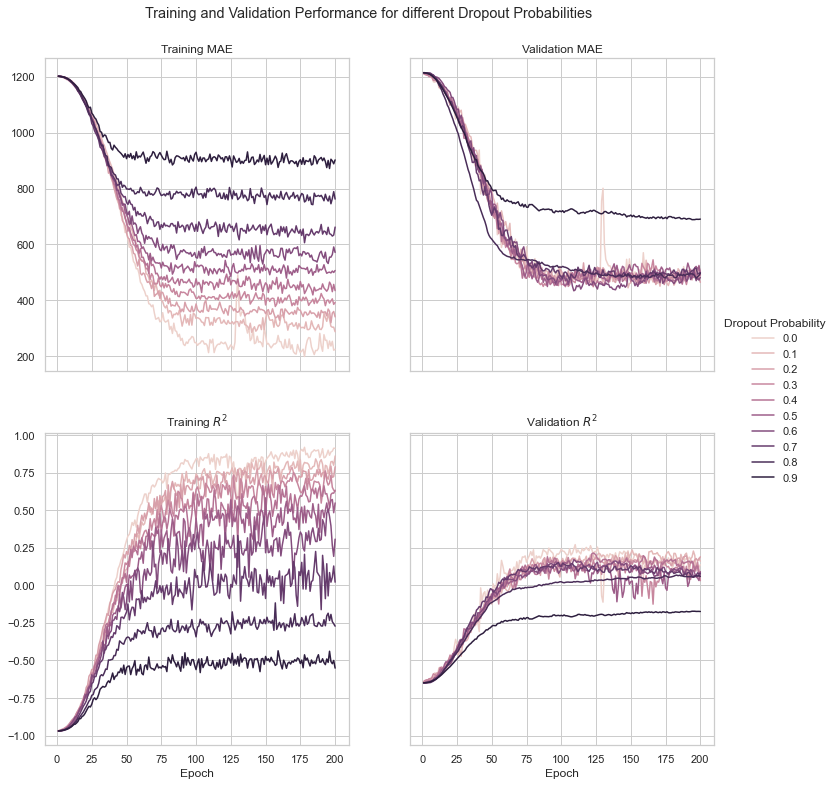
\includegraphics[width=0.9\textwidth]{dropout_performance.png}
  \caption{Impact of Dropout Probability on Training and Validation Performance}
  \label{fig:dropout}
\end{figure}
